% Created 2023-03-12 Вс 02:18
% Intended LaTeX compiler: pdflatex
\documentclass[PI, VKR]{HSEUniversity}
                \Year{\the\year{}}
                                \supervisor{к.т.н.}{доцент кафедры информационных технологий в бизнесе НИУ ВШЭ-Пермь}{А. В. Бузмаков}
\Abstract{В данной работе проведен анализ этичности разных компаний.

В первой главе находится описание используемых алгоримов.

Во второй главе представлено проектирование системы.

В третьей главе представлена реализация системы.

В четвертой главе представлено тестирование работы системы.

Количество страниц -- \pageref*{pg:end}, количество иллюстраций -- \TotalValue{totalfigures}, количетсво таблиц -- \TotalValue{totaltables}.
}
\author{Соломатин Роман Игоревич}
\date{\today}
\title{Разработка сайта для автоматического сбора, анализа и визуализации информации по этичности компаний}
\hypersetup{
 pdfauthor={Соломатин Роман Игоревич},
 pdftitle={Разработка сайта для автоматического сбора, анализа и визуализации информации по этичности компаний},
 pdfkeywords={},
 pdfsubject={},
 pdfcreator={Emacs 28.2 (Org mode 9.6.1)},
 pdflang={Russian}}
\usepackage{biblatex}
\addbibresource{~/Desktop/notes/org/bibliography.bib}
\begin{document}

\maketitle

\chapter*{Введение}
\label{sec:orgef29acf}
Этика компаний – это разделяемые всеми сотрудниками организации правила и нормы, ценности и убеждения, манера общения и другие факторы, которые регламентируют поведение и взаимодействии членов компании. Существует 3 уровня этики компаний\autocite{smirnova_biznesetika_2021}:
\begin{enumerate}
\item мировой -- отвечает за увеличение общественного благосостояния, обеспечение рабочих мест, научно-технические инновации и модернизацию производственных процессов и т. д.
\item макроуровень -- отвечает за принципы рыночной конкуренции, информационной прозрачность и равнодоступности для всех участников рынка и т. д.
\item микроуровне -- отвечает за доверие и отсутствие дискриминации в отношениях между контрагентами, между сотрудниками и менеджерами, морально-нравственный климат в организации и т. д.
\end{enumerate}
В данной работе будет рассматриваться этика на микроуровне.

Этичность компаний уже давно вызывает озабоченность, особенно их поведение в спорных ситуациях и предоставление услуг, ориентированных на клиента. В последние годы все большее внимание уделяется оценке этичности компаний\autocites{mure_esg_2021}[][]{semenko_korporativnaya_2022}[][]{kudryavceva_korporativnosocialnaya_2016}, особенно в банковском секторе и через призму экологических, социальных и управленческих факторов (ESG). Необходимость в таких оценках становится все более острой по мере того, как общество продолжает бороться с последствиями неправомерных действий корпораций и более широким воздействием корпоративной деятельности на общество и окружающую среду.

В настоящее время существует несколько сервисов, которые призваны оценивать этику компании на основании финансовых показателей\footnote{\url{https://kontur.ru/expert}, \url{https://www.esphere.ru/products/spk/financial}} и судебных дел\footnote{\url{https://proverki.gov.ru/portal/public-search}}. Это привело к ситуации, когда отдельные лица должны проводить свои собственные исследования, чтобы определить насколько этична компания. Это часто включает в себя просмотр отзывов с различных веб-сайтов, что может занять много времени и не всегда может дать исчерпывающую или точную картину, так как не включает в себя качество обслуживания.

Для решения этой проблемы реализована система, которая собирает и анализирует отзывы потребителей с различных веб-сайтов, чтобы дать более полную и точную оценку этической практики компании. Затем собранные данные анализируются с помощью различных методов, таких как обработка естественного языка и машинного обучения, для выявления закономерностей и тенденций, связанных с этической практикой компании. Полученный анализ может быть использован для разработки более надежной и достоверной системы оценки этичности компаний.

Объект исследования – взаимодействие компаний с клиентами.

Предмет исследования – программные средства для оценки этичности на основе взаимодействия компаний с клиентами.

Цель работы – создание системы для оценки этичности компаний.

Исходя из поставленной цели, необходимо:

\begin{enumerate}
\item Провести анализ предметной области и требований
\item Реализовать систему
\item Провести тестирование системы
\end{enumerate}

Этап анализа должен:
\begin{enumerate}
\item Анализ предметной области
\item Анализ требований к системе
\item Анализ существующих алгоритмов
\end{enumerate}

Этап проектирования должен включать:
\begin{enumerate}
\item Проектирование серверной части
\item Проектирование модели для определения этичности
\item Проектирование клиентской части приложения
\end{enumerate}

Этап реализации должен включать:
\begin{enumerate}
\item Описание сбора данных
\item Реализации модели
\item Реализации серверной части
\item Реализации клиентской части
\end{enumerate}

Этап тестирования должен включать:
\begin{enumerate}
\item Тестирование модели
\item Тестирование серверной части
\item Тестирование клиентской части
\end{enumerate}

В ходе выполнения анализа, проектирования и реализации приложения используется объектно-ориентированный подход. Результаты анализа и решения задач проектирования формализуются с помощью диаграмм \texttt{UML}. При разработке базы данных используется реляционная СУБД \texttt{PostgreSQL}, а серверная часть приложения реализуется на языке python с помощью фреймворка \texttt{FastApi}, а алгоритмы анализы текста будут использовать методы машинного обучения.
\chapter{Анализ предметной области}
\label{sec:org9bf84bf}
В данной главе представлен аналитический обзор оценок этичности компаний и алгоритмов машинного обучения, а также обзор существующих программных решений для поставленной проблемы.

Анализ предметной области следует разделить на следующие пункты:
\begin{enumerate}
\item анализ процесса определения этичности компаний сейчас позволяет понять, как этот процесс сейчас происходит и как его лучше всего автоматизировать;
\item анализ оценок этичности компаний для того, чтобы в дальнейшем определить этичность компаний;
\item анализ существующих решений выполняется с целью выделения их сильных и слабых сторон по отношению к решаемой проблеме и обоснования необходимости разработки нового средства, подходящего под регламент задач;
\item анализ алгоритмов позволяет понять с помощью каких алгоритмов можно найти полезную информацию в текстах;
\item анализ требований к системе позволит выделить функциональные и не функциональные требования.
\end{enumerate}
\section{Анализ определения этичности компании}
\label{sec:orgb069323}
Сейчас процесс поиска этичной компании выгладит следующим образом: сначала ищутся компании, которые предоставляют желаемые услуги. Далее они изучаются, чтобы определить их этичность. Этот процесс включает в себя:
\begin{enumerate}
\item просмотр отчетности компании
\item анализ ее финансовой деятельности
\item изучение информации о социальной ответственности
\end{enumerate}

Для этого они обращаются к различным источникам информации, таким как веб-сайты компаний, рейтинговые агентства, исследовательские организации и другие источники. Потом, изучаются социальные сети компании или отзывы пользователей на разных сайтах, форумах и социальных сетях, чтобы получить дополнительную информацию и оценить общее мнение о компании. После изучения каждой компании люди выбирают ту, которую они считают наиболее этичной и социально ответственной. Блок-схема данного поиска рис. \ref{fig:as_is}. Важным фактором для определения этичности компании может быть ее социальная ответственность, устойчивость бизнеса и соблюдение норм и стандартов в области финансовой деятельности.

В целом, процесс поиска компаний и определения их этичности может быть длительным и требует серьезного подхода. Люди могут использовать различные источники информации, чтобы сделать осознанный выбор и инвестировать свои деньги в компанию, которая соответствует их ожиданиям и требованиям.
\begin{figure}[h]
\centering
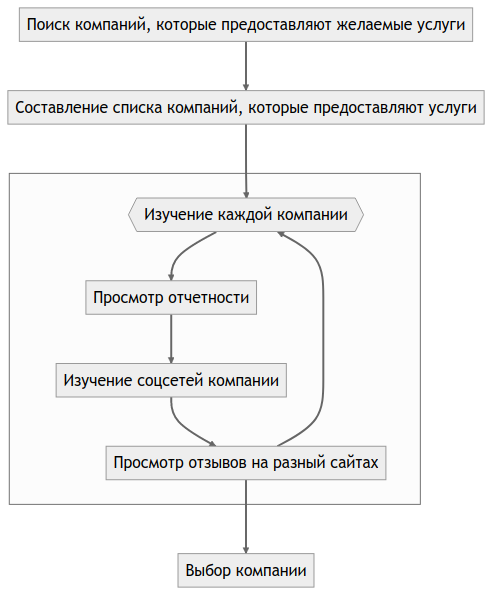
\includegraphics[width=0.6\textwidth]{img/mermaid/as_is.png}
\caption{\label{fig:as_is}Диаграмма того, как сейчас происходит поиск компании}
\end{figure}

\section{Анализ оценок этичности компаний}
\label{sec:org98d8f29}
Оценка этики компании -- это не одноразовый процесс, а скорее непрерывная попытка понять и оценить действия, политику и практику компании с течением времени. Это включает в себя рассмотрение соблюдения компанией отраслевых этических стандартов и передовой практики, а также мониторинг любых изменений в этической позиции компании с течением времени. Кроме того, участие в диалоге с компанией и консультации с организациями, специализирующимися на оценке корпоративной ответственности могут дать ценную информацию об этических практиках компании.

Компаниям важно оставаться этичными, так как на долгосрочной перспективе это приносит большую прибыль и улучшает показатели бизнеса, чем неэтичный способ ведение бизнеса\autocites{climent_ethical_2018}[][]{mure_esg_2021}. Насколько этична компания можно рассматривать с двух сторон, самой компании и их клиентов. Со стороны компаний можно выделить факторы, которые можно получить из их отчетности:
\begin{itemize}
\item количество капитала, чтобы они не могли обанкротиться;
\item какое влияние они вносят на окружающую среду;
\item куда идут инвестиции\autocite{harvey_ethical_1995}.
\end{itemize}
Для пользователей одними из ключевых факторов можно выделить:
\begin{itemize}
\item качество пользовательского сервиса\autocite{brunk_exploring_2010};
\item насколько навязчивые услуги компании\autocite{mitchell_bank_1992}.
\end{itemize}

В данной работе этичность компаний будет определяться по отзывам клиентов, которые освещают проблемы качества услуг и качество сервиса, и на основе отчетности компаний, что позволит полностью осветить проблему. Для анализа текстов будут использоваться алгоритмы машинного обучения.
\section{Анализ существующих решений}
\label{sec:org2334d65}
Сейчас данные об этичности компаний можно получить из агрегаторов отзывов и отчётности компаний. Агрегаторы отзывов позволяют собрать информацию о клиентском обслуживании, а отчетность компаний о положении дел в целом. Но сейчас не существует способов, как можно оценить все вместе.
\section{Алгоритмы для анализа текста}
\label{sec:org739ed70}
Алгоритмы машинного обучения для анализа текста получили широкое распространение для извлечения информации из неструктурированных данных с помощью больших помеченных наборов данных. Среди различных используемых методов несколько алгоритмов оказались особенно эффективными в этой области. К ним относятся мешок слов\autocite{harris_distributional_1954}, TF-IDF\autocite{jones_karen_sparck_statistical_1972}, Word2Vec\autocite{mikolov_distributed_2013}, ELMO\autocite{peters_deep_2018}, GPT\autocite{radford_language_2019} и BERT\autocite{devlin_bert_2019}. Каждый из этих алгоритмов обладает уникальными характеристиками, которые делают их хорошо подходящими для определенных приложений.

Модель {}<<Мешок слов>>{} представляет текстовые данные путем присвоения уникального номера каждому слову в документе. Этот метод прост в реализации, но не учитывает порядок слов в предложении. С другой стороны, модель TF-IDF представляет текстовые данные, учитывая как частоту слова в документе (TF), так и его редкость во всех документах корпуса (IDF). Этот подход может быть использован для определения важности слова в данном документе и обычно используется в задачах поиска информации и обработки естественного языка, но он не понимает контекста слов.

Word2Vec использует векторное представление слов, что позволяет алгоритму улавливать значение слов в сходных контекстах. Это позволяет более точно и изощренно представлять взаимосвязи между словами, что приводит к повышению производительности в таких задачах, как классификация текста и анализ настроений.

ELMO, GPT и BERT, с другой стороны, основаны на архитектуре трансформеров, в которой каждое предложение представлено вектором чисел, обычно известным как вложение. Такое представление позволяет получить более полное и целостное понимание текста, поскольку оно учитывает контекст всего предложения или текста.

Из этих алгоритмов BERT считается наиболее продвинутым и мощным, поскольку он способен учитывать контекст всего предложения или текста, в то время как GPT и ELMO рассматривают только односторонний контекст. Это позволяет BERT достигать самых современных результатов в широком спектре задач анализа естественного языка.

Таблица результата сравнения моделей \ref{tbl:model_compare}.

\begin{table}[h]
\caption{\label{tbl:model_compare}Сравнение моделей}
\centering
\begin{tabular}{|c|c|c|}
\hline
Модель & Вектор слов & Контекст\\[0pt]
\hline
Мешок слов & зависит от количества слов & нет\\[0pt]
\hline
TF-IDF & зависит от количества слов & очень слабо\\[0pt]
\hline
Word2Vec & не зависит от количества слов & слабо\\[0pt]
\hline
ELMO & не зависит от количества слов & однонаправленный\\[0pt]
\hline
GPT & не зависит от количества слов & однонаправленный\\[0pt]
\hline
BERT & не зависит от количества слов & двунаправленный\\[0pt]
\hline
\end{tabular}
\end{table}

\subsection{BERT}
\label{sec:orge46c100}
BERT \autocite{devlin_bert_2019} (Bidirectional Encoder Representations from Transformers) -- это нейросетевая языковая модель, которая относится к классу трансформеров. Она состоит из 12 «базовых блоков» (слоев), а на каждом слое 768 параметров.

На вход модели подается предложение или пара предложений. Затем разделяется на отдельные слова (токены). Потом в начало последовательности токенов вставляется специальный токен \texttt{[CLS]}, обозначающий начало предложения или начало последовательности предложений. Пары предложений группируются в одну последовательность и разделяются с помощью специального токена \texttt{[SEP]}, затем к каждому токену добавляется эмбеддинг, показывающий к какому предложению относится токен. Потом все токены превращаются в эмбеддинги \ref{fig:inputemebeddings} по механизму описаному в работе \autocite{vaswani_attention_2017}.

\begin{figure}[h]
\centering
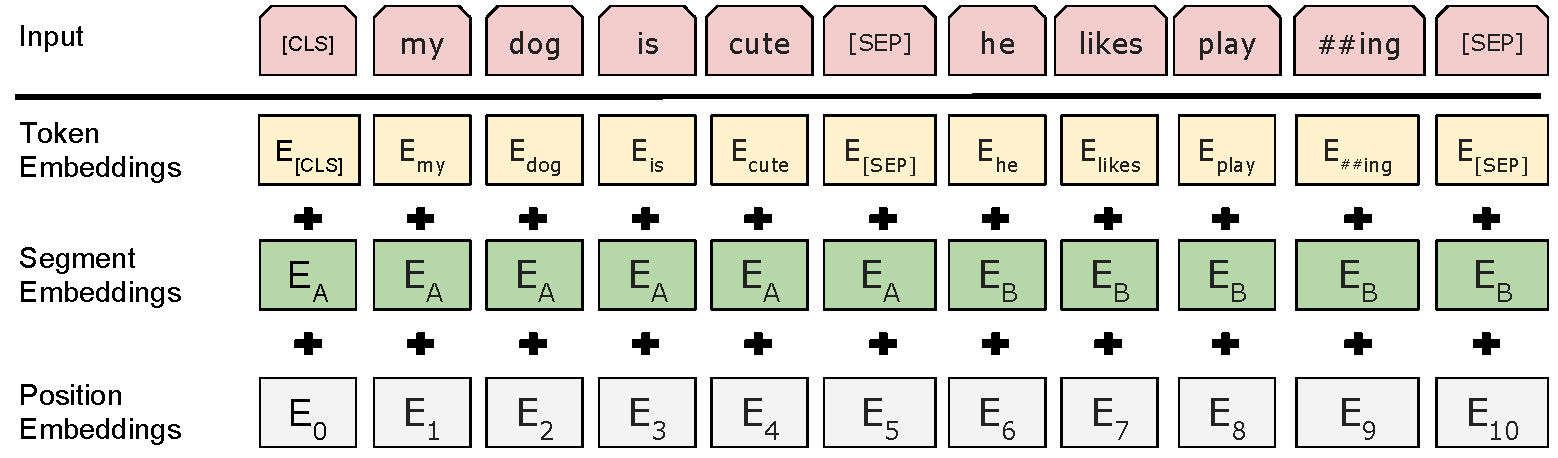
\includegraphics[width=.9\linewidth]{img/Input_Emebeddings.pdf}
\caption{\label{fig:inputemebeddings}Пример ввода текста в модель}
\end{figure}

При обучении модель выполняет на 2 задания:
\begin{enumerate}
\item Предсказание слова в предложении

Поскольку стандартные языковые модели либо смотрят текст слева направо или справа налево \ref{fig:BERT_comparisons}, как ELMo\autocite{peters_deep_2018} и GPT\autocite{radford_language_2019}, они не подходят под некоторые типы заданий. Так как BERT двунаправленный, у каждого слова можно посмотреть его контекст, что позволит предсказать замаскированное слово.

\begin{figure}[h]
\centering
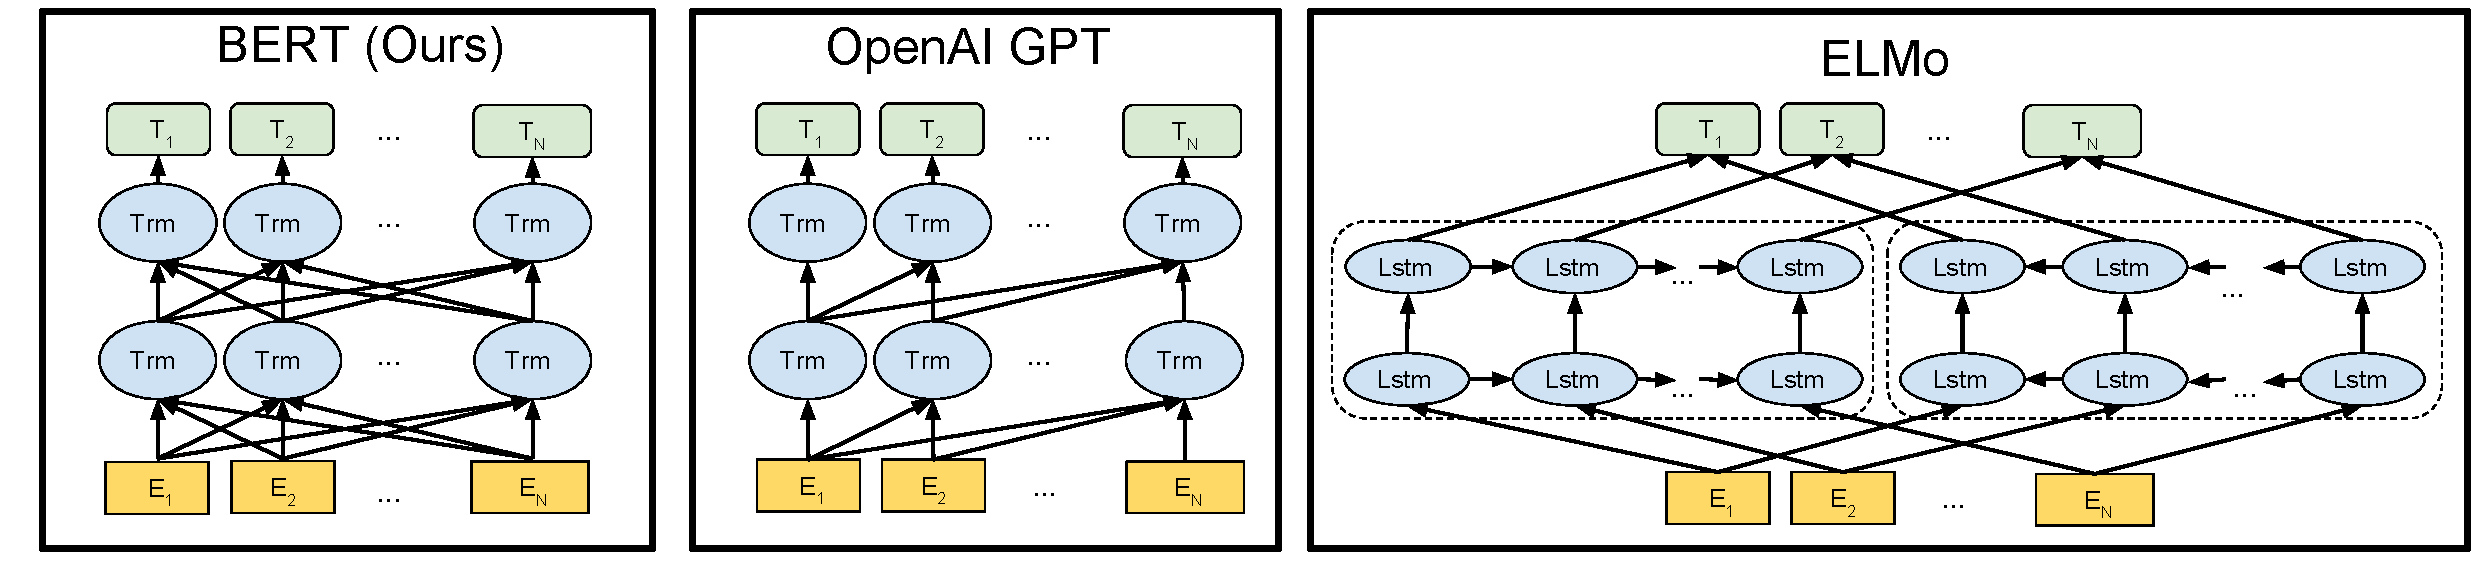
\includegraphics[width=.9\linewidth]{img/BERT_comparisons.pdf}
\caption{\label{fig:BERT_comparisons}Сравнение принципов работы BERT, ELMo, GPT}
\end{figure}

Это задание обучается следующим образом -- 15\% случайных слов заменяются в каждом предложении на специальный токен \texttt{[MASK]}, а затем предсказываются на основании контекста. Однако иногда слова заменяются не на специальны токена, в 10\% заменяются на случайный токен и еще в 10\% заменяются на случайное слово.

\item Предсказание следующего предложения

Для того чтобы обучить модель, которая понимает отношения предложений, она предсказывает, идут ли предложения друг за другом. Для этого с 50\% вероятностью выбирают предложения, которые находятся рядом и наоборот. Пример ввода пары предложений в модель \ref{fig:bert_pretrainin}.

\begin{figure}[hbp]
\centering
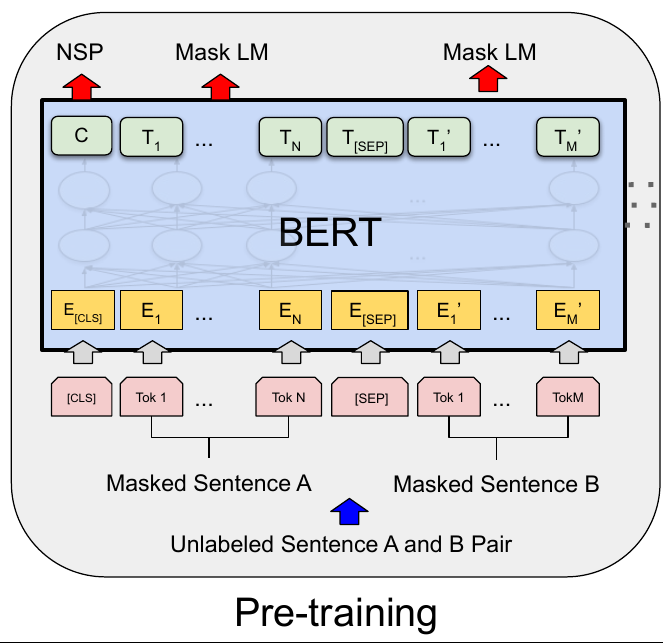
\includegraphics[width=0.6\textwidth]{img/bert_pretrainin.png}
\caption{\label{fig:bert_pretrainin}Схемам работы BERT}
\end{figure}
\end{enumerate}
\subsection{Sentence BERT}
\label{sec:org802eec5}
Sentense BERT \autocite{reimers_sentence-bert_2019} -- это модификация предобученных моделей BERT, которая использует 2 модели BERT, затем усреднят их выходы, а после с помощью функции ошибки выдаёт результат. Схема работы модели \ref{fig:sbert}.
\begin{figure}[hbp]
\centering
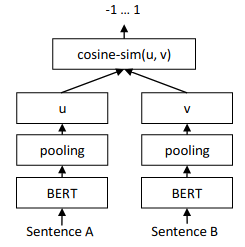
\includegraphics[width=0.6\textwidth]{img/sbert.png}
\caption{\label{fig:sbert}Схема работы SBERT}
\end{figure}
Основное преимущество данной модели над классическим BERT: эмбеддинги предложений можно сравнивать друг с другом независимо и не пересчитывать их пару каждый раз. Например, если для поиска похожих предложений из 10000 для обычного BERT потребуется 50 миллионов вычислений различных пар предложений, и это займёт 50 часов, то Sentense BERT рассчитает эмбеддинг каждого предложения отдельно, потом их сравнит. Такой способ рассчета ускоряет работу программы до 5 секунд.
\section{Анализ требований к системе}
\label{sec:orgf52b97a}
Исходя из интервью с пользователями система должна уметь:
\begin{enumerate}
\item Показывать историю изменений индекса с возможностью фильтровать по:
\begin{enumerate}
\item годам
\item отраслям компаний, с возможностью множественного выбора
\item компаниям, с возможностью множественного выбора
\item моделям, с возможностью множественного выбора
\item источникам, с возможностью множественного выбора
Также, надо агрегировать значения индекса по годам и кварталам
\end{enumerate}
\item Анализировать тексты для построения индекса этичности
\item Сохранять тексты для последующего анализа другими методами
\end{enumerate}
На основе описания функциональных требований была создана диаграмма вариантов использования, которая представлена на рисунке \ref{fig:usecasefull}.

\begin{figure}[h]
\centering
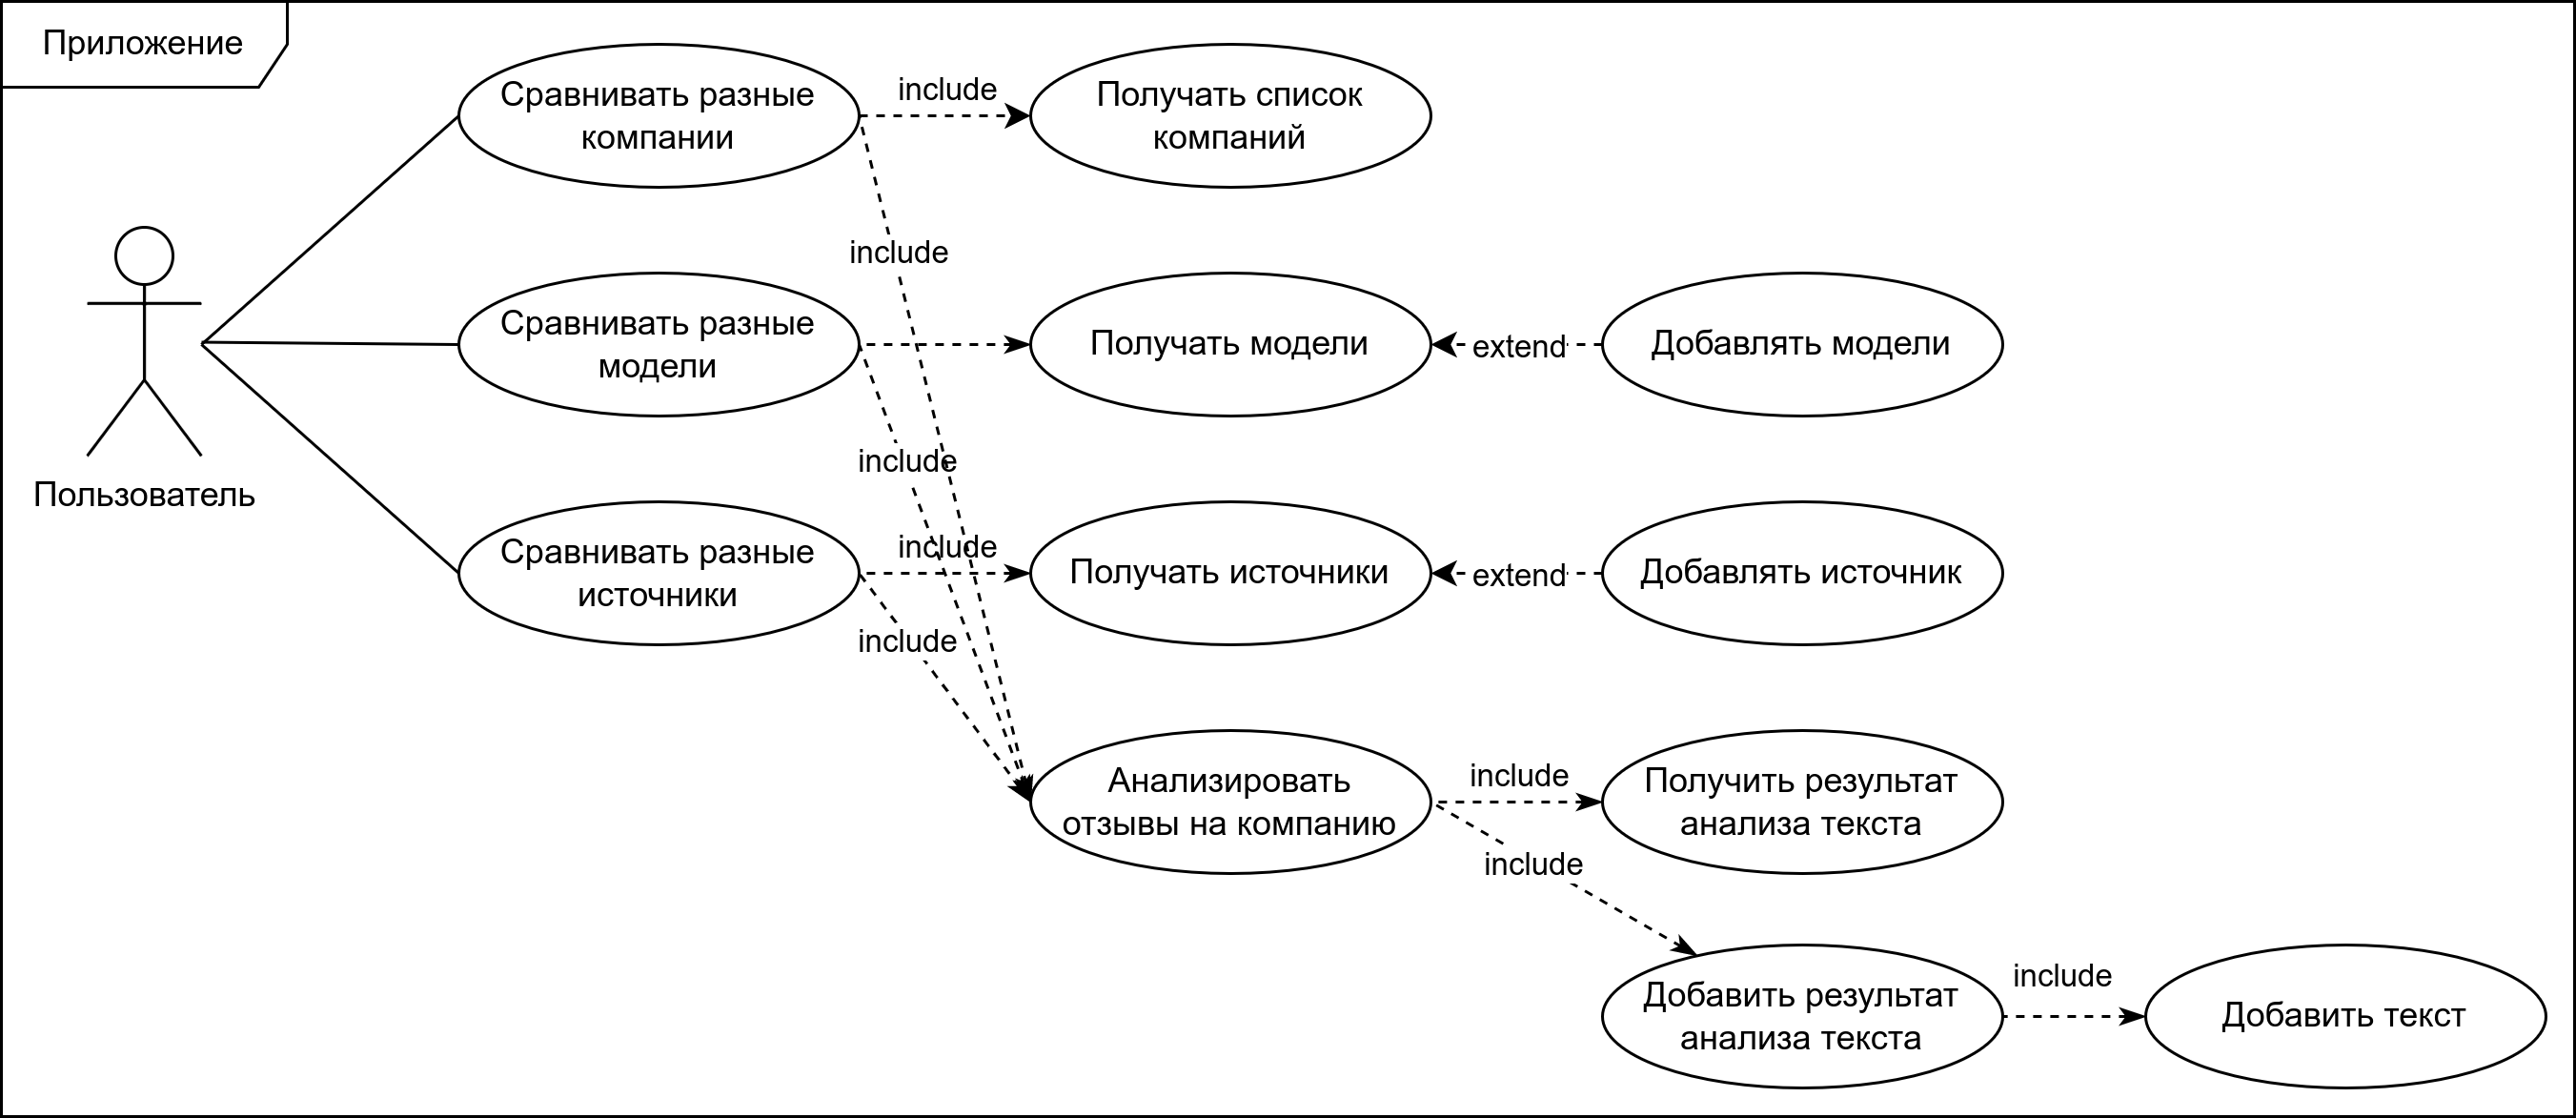
\includegraphics[width=\textwidth]{img/use-case.png}
\caption{\label{fig:usecasefull}Диаграмма вариантов использования}
\end{figure}
Также было сказано, что построение графика не должно занимать больше секунды.
\section{Выводы главы}
\label{sec:orgcd2ed29}
\chapter{Проектирование системы}
\label{sec:org473b6c7}
тут текст
\section{Проектирование базы данных}
\label{sec:org846e47e}

\section{Проектирование архитектуры системы}
\label{sec:org11dbf90}
\subsection{Проектирование серверной части}
\label{sec:org5d98d92}
\subsubsection{Парсер}
\label{sec:org43d7c57}
\subsubsection{Модель}
\label{sec:org14ba912}
\subsection{Проектирование клиентской части}
\label{sec:orgaf6af09}
\chapter{Реализация системы}
\label{sec:org2f67282}
\section{Реализация серверной части}
\label{sec:orge776953}
\subsection{Реализация API}
\label{sec:orgcd3fa49}
\subsection{Реализация парсера banki.ru}
\label{sec:org5c46097}
\subsection{Реализация парсера sravni.ru}
\label{sec:org67eff43}
\subsection{Реализация модуля обработки текста}
\label{sec:org1708fa3}
\subsection{Дообучение модели}
\label{sec:org1d52f9f}
\section{Реализация клиентской части}
\label{sec:org7cc26d7}
\chapter{Тестирование системы}
\label{sec:org48983d0}
\chapter*{Заключение}
\label{sec:orgb5a41a4}
\putbibliography
\appendix
\end{document}
